\chapter{Metodologi}

Pada bab ini penulis menjelaskan mengenai metodologi yang digunakan selama pengerjaan tugas akhir.

\begin{figure}[H]
	\begin{centering}
		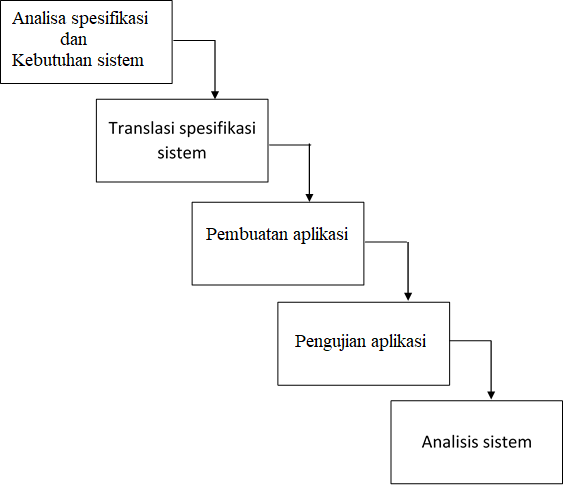
\includegraphics[scale=0.7]{metodologi_proposal}
		
		\caption{Metodologi.}
	\end{centering}
\end{figure}

\section{Analisa spesifikasi dan Kebutuhan sistem}

Menganalisa spesifikasi-spesifikasi pada teka-teki sudoku, lalu membuat kebutuhan dari aplikasi sistem yang akan mengeluarkan \textit{use case} aplikasi.

\section{Translasi spesifikasi sistem}

Spesifikasi yang sudah di dapat diubah dalam bentuk logika proposisi lalu dijadikan dalam bentuk CNF.

\section{Pembuatan aplikasi}

Data yang telah didapatkan akan diubah dalam model formal . . . .

\section{Pengujian aplikasi}

Model formal yang telah dibuatkan akan diverifikasi menggunakan . . . .

\section{Analisis sistem}

Hasil verifikasi akan dianalisis . . . .